\documentclass[10pt, a5paper, twoside]{NGPLS}
\author{周造麟}
\title{30 天 LaTeX}

%\usepackage{luatexja-fontspec}
%\setmainjfont{jf-openhuninn-1.1.ttf}
\usepackage{xeCJK}
\setCJKmainfont{jf-openhuninn-1.1.ttf}

\setlength{\parindent}{0pt}
\linespread{1.35}
\pagenumbering{arabic}

\usepackage[pipeTables, strikeThrough = true]{markdown}
\markdownSetup{fencedCode = true}
\markdownSetup{
  renderers = {
    image = {\begin{figure}[!htb]
      \centering
      \includegraphics[width = .8\linewidth]{#3}%
      \ifx\empty#4\empty\else
        \caption{#4}\label{fig:#1}%
      \fi
    \end{figure}},
    }
}
\usepackage{graphicx}
\graphicspath{{fig/}}

\usepackage{etoolbox}
%\AtBeginEnvironment{itemize}{\vskip6pt}
\AtBeginEnvironment{tabular}{\vskip6pt}
\AfterEndEnvironment{tabular}{\vskip6pt}

\usepackage[svgnames]{xcolor}
%\definecolor{LightGray}{gray}{0.9}

\usepackage{minted}
%\usemintedstyle{borland}

\usepackage{xurl}
\usepackage[breaklinks=true]{hyperref}
\urlstyle{same}
\hypersetup{
colorlinks=true,
linkcolor=blue,
urlcolor=cyan,
hyperindex = false
}

%\setlength{\parskip}{0.1\baselineskip}

\usepackage{amsmath}
\usepackage{amsfonts}
\usepackage{amssymb}

\usepackage{geometry}
\geometry{top=1.5cm, outer=1.75cm, inner=1.5cm, bottom=1.5cm, footskip=24pt}

\begin{document}%\color{Gold}\pagecolor{black}
\maketitle
\tableofcontents\newpage
\begin{markdown}
#30天 LaTeX 挑戰 Day 1 編譯引擎、格式、發行版與編輯器(上)

------

##巨集

巨集是指將一連串的指令換為以一串文字替代,類似將往(往前+右轉)X4 換成話正方形一樣,LaTeX 有許多的巨集包(以下用 Package 代稱)可供使用,如有特殊需求也可以自行撰寫。

##編譯引擎與格式的差異

LaTeX 是由兩個部分所組成的,一個是編譯引擎( Engine )一個是格式,格式簡單來說是一個龐大的巨集,裡面將基本命令封裝成的高級命令,而編譯引擎則是負責命令轉成 PDF 的工作。

##編譯引擎與格式

###格式
目前據我所知有以下兩種格式

* Plain TeX
* LaTeX

Plain TeX 是高德納教授自行編寫的,但由於對普通人還是太過艱澀,所以之後 Leslie Lamport 編寫了 LaTeX,使得像我這樣的普通人也可以享受 TeX 帶來的方便性。 

我並沒有使用過 Plain TeX 這個格式,所以本篇所有的程式碼都是基於 LaTeX 這個格式的。

###編譯引擎
據我所知有以下這幾種

* TeX
* pdfTeX
* xeTeX
* LuaTeX
* pTeX & upTeX

#### TeX

當時的高德納教授正準備出版他的著作《The Art of Computer Programming》,但他覺得書商將他的著作排得太難看了,於是他便寫出了 TeX 來為自己的著作排版。

####pdfTeX

一開始 TeX 只能產生 dvi 檔,如果需要 pdf 檔得使用 dvips + ps2pdf 或 dvipdf 等,用久了難免會覺的不方便,於是就有人對 TeX 進行了改進,使 TeX 能夠直接的產生 Pdf 檔,而這改進過的引擎就被命名為 pdftex。

####XeTeX 

隨著時代的進步,TeX 並沒有消逝在歷史的洪流中,但對於日新月異的電腦科學來說,TeX 所支持的字體技術及編碼過於的老舊,於是便開發了支持 Opentype, Truetype, Unicode 的 XeTeX,並可以直接調用系統字體。

####LuaTeX

後來有人希望可以建立一個開放且可配置的 TeX 環境,於是就將 Lua 加進了 pdfTeX 裏成為了 LuaTeX。

LuaTeX 可在文章中直接使用 Lua 來改變排版細節,也支持 Unicode 編碼及現代的字型技術。

#### pTeX \& upTeX

這算是一個比較特殊的分枝,在 TeX 傳入日本後,因為 TeX 本身不支持非拉丁語系的文字,於是日本人便將 TeX 依照自己的需求改進,最終的產物就是原生支持日文的 pTeX(但只支持特定編碼,upTeX 才支持 unicode 編碼) ,除了原生支持日文外也支持豎排文章。

\end{markdown}\newpage
\begin{markdown}
#30天 LaTeX 挑戰 Day 2 編譯引擎、格式、發行版與編輯器(下)
##發行版

TeX 發行版可以說是將編譯引擎、格式與 Pacakge 都集中到一起的集合,通常我們不會單獨下載編譯引擎與格式,而是會直接下載發行版。我所知發行版有以下三種。

* TeX Live
* MiKTeX
* MacTeX

###TeX Live

由 TUG(TeX User Group)維護的發行版,可以說是目前最活躍的 TeX 發行版,但我並不是使用這個發行版,關於使用方法可以參考使用手冊<https://tug.org/texlive/doc.html>。

###MiKTeX

MiKTeX 的哲學是夠用就好(Just Enough TeX),一開始安裝時只需要下載基本的 Package 即可,隨後如果有缺失的 Package 便會在編譯前下載(On The Fly),如果你不想裝龐大的 TeX 發行版可以考慮這個。

###MacTeX

MacTeX 實際上是對 TeX Live 進行改造,加入許多對於 MacOS 系統的優化,適合想在 MacOS 上使用 TeX 卻又不想搗鼓太多的人。

##編輯器

編輯器說穿了就是文本編輯器,如果你對於 LaTeX 非常熟悉,不用下載特別的編輯器也可以進行 LaTeX 的撰寫。不過想當然的,專門為 LaTeX 開發的編譯器一定能讓你事半功倍。


小弟推薦 texmaker,是一個專為編輯 tex 文件所開發的開源軟體,有自動補全命令、顯示文章架構與原始碼和PDF並排的功能,我個人使用下來的經驗是非常美好的。但沒有什麼東西是完美的,texmaker 需要設定比較多的選項才能順利的編譯 tex 文件。

下一章就要教大家如何建構環境了。
\end{markdown}\newpage
\input{3}\newpage
\begin{markdown}
#30天 LaTeX 挑戰 Day 4 中文環境配置

來到了第四天,在將發行版與編譯器都下載好之後終於要進入到使用中文了,以下提供數種支持中文的方式。

##PdfLaTeX + CJK

在 Preamble 中加入`\usepackage{CJKutf8}`並且在需要使用到中文的部分使用`\begin{CJK}{UTF-8}{字體}......\end{CJK}`就可以使用中文了,下面有一個小小的範例

```latex
\usepackage{CJKutf8}
% bsmi = 明體
% bkai = 楷書
\begin{CJK}{UTF-8}{bsmi}
這裡就可以用中文了喔
\end{CJK}
```

但這種方法可以使用的中文字體必須是 TeX 發行版自帶的中文字體,在字體的選擇上有一定的局限性。

##XeLaTeX + fontspec 的土炮用法

在 XeLaTeX 的環境下使用`latex\usepackage{fontspec}`並宣告新的字體`latex\newfont\swich{Font}`,然後就可以在文本區中需要中文的地方用\{\swich 中文\}的方式打出中文了。

##XeLaTeX + CTeX

CTeX 是一套由中國人開發的巨集,但其實他本身並不提供中文支持,只是它會幫你根據你的編譯引擎設定好巨集,除此之外 CTeX 還一並提供了符合中文排版的文件格式、預先定義好的中文字體,但不知道為什麼,這套對 Mac OS 的兼容性並不好。

```latex
\documentclass[•]{•}
\usepackage{ctex}
\begin{document}
我可以用中文了
\end{document}
```

|名稱|用途|
|-----|-----|
|ctexart|簡單的幾頁文件|
|ctexrep|報告|
|ctexbook|書籍|
|ctexbeamer|投影片|

^提供的文件格式

##XeLaTeX + xeCJK

這是 ctex 在 XeLaTeX 的環境下使用的中文支持方案,一些常用的設定如下。

```latex
\usepackage{xeCJK}%匯入巨集
\setCJKmainfont[可選參數]{字體名}%設置主要字體
\setCJKfallbackfont[可選參數]{字體名}%設置備用字體
```

##LuaLaTeX + luatexja

這是必須使用 LuaLaTeX 時才會用到的配置,不然我主要是使用 xeCJK

```latex
%\documentclass[•]{•}
%加-fontspec 才可以設定字體
\usepackage{luatexja-fontspec}
\setmainjfont{Font}
%然後就可以使用中文了
```

##總結

使 LaTeX 支持中文的方法不只一種,可以依照自己的需求尋找最適合的方式,我推薦 XeLaTeX + xeCJK 或 LuaLaTeX + luatexja 的方式,其他就讓它留在歷史的洪流中吧。

\end{markdown}\newpage
\input{5}\newpage
\begin{markdown}
#30天 LaTeX 挑戰 Day 6 文檔結構
---

本篇文章是要介紹 LaTeX 的文檔節構,LaTeX 文檔可以分成兩個大部分:導言區與文本區,這兩個部分是拿來幹嘛的呢?答案都在本篇內。

##導言區

導言區指的是檔案內 \begin{document} 前的部分,通常我們會在這裡引入需要的 package、選擇文件的類別、定義一些需要的參數、命令,你可以簡單的理解為定義模板,或理解為 HTML 的 \<HTML\> 標籤。

```latex
\documentclass[]{}
%導言區
\begin{document}
%文本區
\end{document}
```
在導言區下列兩個命令是最為重要的

* \documentclass[]{}
* \usepackage{}

前者是決定文件的類別,後者是使用巨集,下表與可選的文件類別

| 文件類別 | 用途 |
| ------ | ------ |
| article | 短文章 |
| report | 多章節的長報告 |
| book | 書籍 |
| beamer | 簡報 |

本篇若未特別說明皆是基於 article 類別

|巨集|用途|
|----|----|
|xeCJK|XeTeX 為編譯引擎的環境下提供中文支持|
|xcolor|使 LaTeX 支持多彩|
|mhchem|化學反應式|
|chemfig|化學結構式|
|Geometry|文件版面|
|tikz|繪圖|
|tcolorbox|好看的 color box|
|listings|程式碼展示|
|graphicx|圖片|
|biblatex|參考文獻管理|
∆常用巨集列表

##文本區

文本區才是文章的內容的所在,文章上會顯示的內容都會被打在這裡。

###標題與目錄

在 LaTeX 預定義的文件類別中,有以下幾種的標題格式被預定義好,只要使用這些命令,就可以利用 \tableofcontent 建立目錄,也可以利用 \listoffigre 與 \listoftable 來建立圖目錄與表目錄

|名稱|說明|深度|
|---|---|---|
|\part{}|部|-1 (在 article 為 0)|
|\chapter{}|章|0(在 article 中未被定義)|
|\section{}|節|1|
|\subsection{}|小節|2|
|\subsubsection{}|小小節|3|
|\paragraph{}|段|4|
|\subparagraph{}|小段|5|

深度在 LaTeX 文件類型的定義中是用來決定該不該被 \tableofcontent 編入目錄的,以下有一些有關的指令

```latex
\setcounter{tocdepth}{2}%設定深度

\section*{}%只要加一個星號就會不編號也不編入目錄

\addcontentsline{toc()/lof/lot}{層級}{名稱}%將未編入目錄的標題標入目錄
```
\end{markdown}\newpage
\begin{markdown}
# 30天 LaTeX 挑戰 Day 7 版面配置

##一些內建的處理

以下是 LaTeX 的文件類別內建的版面配置

|選項|含義|
|-----|-----|
|a4paper|設定紙張大小為a4|
|a5paper|設定紙張大小為a5|
|twoside|雙面模式|
|twocolumn|雙欄模式||
|landscape|將紙張旋轉90度|
|參數|含義|
|paperheight|紙張高度|
|paperwidth|紙張寬度|

選項只需要放在`\documentclass[]{}`的中括號內即可,但下面的參數需要利用`\setlength{參數}{數值}`的方式修改。

```latex
\documentclass[a4paper,landscape]{article}
and
\setlength{\paperheight}{value}
\setlength{\paperwidth}{value}
```

##邊界

邊界可以利用 geometry package 來設定

```latex
\usepackage[key1=value, key2=value]{geometry}
or
\usepackage{geometry}
\geometry{key1=value, key2=value}
```

下表有一些常用的 key

|Key|含義|
|-----|-----|
|top|上邊界|
|bottom|下邊界|
|left|左邊界|
|right|右邊界|
|outter|雙頁模式下的右側邊界|
|inner|雙頁模式下的右側邊界|

##各種距離

這裡要介紹的距離有

* parskip
* parindent
* leftskip
* rightskip
* baselineskip
* lineskip

###parskip

parskip 是指 LaTeX 在兩個段落中加入的空白

```latex
\lipsum[][50]

\lipsum[][50]

\parskip 2cm \lipsum[][50]

\lipsum[][50]
```

可以看到段落間的距離變了

###parindent

parindent 是指段落前的縮進

```latex
\setlength{\parindent}{15pt}
ewjriwerflnioweor
```

但 LaTeX 會將標題後的段落視為引言,引言是不會縮排的

###leftskip & rightskip

這是調整兩邊縮排的

###baselineskip & lineskip

這是跟行距有關的兩個選項,baselineskip 是指兩行字基線的距離,是透過 $font size \times 1.2 \times \linespread{value}$ 得出的,若要在文本區內更改,需要使用 `\selectfont` 命令。

```latex
\setlength{\baselineskip}{12pt}\selectfont
AAAAAA

AAAAAA
\setlength{\baselineskip}{24pt}\selectfont
AAAAAA

AAAAAA
```

lineskip 則是在上下兩條基線超過 baselineskip 時兩行之間的距離,
如果要調整行距,建議使用 setspace package 提供的 `\singlespacing、\onehalfspacing 、\doublespacing` 命令,或者利用 `\linespread{vaule}` 設定行距。

\end{markdown}\newpage
\begin{markdown}
#30天 LaTeX 挑戰 Day 8 字體與字型

-----

來到了第八天,本篇要講的是 LaTeX 的字體與字型的設定。

##字型

###字體大小

LaTeX 預設內文字體是 10pt 並提供了 11 & 12 pt 可供使用,並且 LaTeX 有預設一些字體大小

|環境|swich|10pt|11pt|12pt|
|-----|-----|-----|-----|-----|
|`\begin{tiny}`|`\tiny` | 5pt | 6pt | 6pt |
|`\begin{scriptsize}`|`\scriptsize` | 7pt | 8pt | 8pt |
|`\begin{footnotesize}`|`\footnotesize` | 8pt | 9pt | 10pt |
|`\begin{small}`|`\small` | 9pt | 10pt | 11pt |
|`預設大小`|`\normalsize` | 10pt | 11pt | 12pt |
|`\begin{large}`|`\large` | 12pt | 12pt | 14pt |
|`\begin{Large}`|`\Large` | 14pt | 14pt | 17pt |
|`\begin{LARGE}`|`\LARGE` | 17pt | 17pt | 20pt |
|`\begin{huge}`|`\huge` | 20pt | 20pt | 25pt |
|`\begin{Huge}`|`\Huge` | 25pt | 25pt | 25pt |

如果想要使用特殊的字體大小可利用`\fontsize{font size}{line skip}\selectfont `


###粗體

使用`\textbf{your word}`或`\bfseries` 來改變字體粗細

```latex
\textbf{Bold} or {\bfseries Bold}
```

###斜體

使用`\textit{your word}`或`\itshape` 來更改文字傾斜。

```latex
\textit{italic} or {\itshape italic}
```

###強調

使用`\emph{Important}`即可

```latex
VERY VERT \emph{IMPORTANT}
```

##字體

由於 LaTeX 支持的字體技術過於久遠,於是這裡所要教學的是在 XeLaTeX 與 LuaLaTeX 的環境下可以用的技巧

###在 xeCJK 上

在 xeCJK 中可以利用`\setCJKmainfont[font features]{font}`來設定主要字體,也可以利用`\newCJKfontfamily[family(可不指定,不指定時等同於switch)]\swich{font}[font features]`來聲明新的字族。

```latex
\setCJKmainfont{TW-Kai}
\newCJKfontfamily\sung{TW-Sung}

標楷體、\sung 宋體
```

###在 luatexja 上

在 luatexja 也是一樣,只不過命令長得不一樣,`\setmainjfont` 與`\newjfontfamily`

```latex
\setmainjfont{TW-Kai}
\newjfontfamily\sung{TW-Sung}

標楷體、\sung 宋體
```
\end{markdown}\newpage
\begin{markdown}
# 30天 LaTeX 挑戰 Day 9 列表與表格

------

##列表

在 LaTeX 中有三種不同的列表環境, 分別是 itemize, enumerate 與 description,這三個在使用上除了輸出結果不同外,其他都是完全相同的。

### itemize

itemize 是最簡單的列表環境

```latex
\begin{itemize}
\item 第一點
\item 第二點
\item 第三點
\end{itemize}
```

只要在環境中利用 `\item` 就可以放置項目符號,如果想要自訂項目符號,只需要像 `\item[]` 這樣指定即可

```latex
\begin{itemize}
\item 第一點
\item[\$]第二點
\item[\#]第三點
\end{itemize}
```

可以看到第二點與第三點的項目符號換成了 \$ 與 \# ,也可以將項目符號換成數字

```latex
\begin{itemize}
\item[1]第一點
\item[2]第二點
\item[2]第三點
\end{itemize}
```

但通常不會有人這樣做,因為可以靠下一個要介紹的列表環境來達成類似的事情。

### enumerate

如同上一段所說, enumerate 的項目符號是連續的數字,如果需要列出有順序的列表,可以考慮使用這個環境。

```latex
\begin{enumerate}
\item 第一點
\item 第二點
\item 第三點
\end{enumerate}
```

如果想要在一個大項目下細分出子項目,可以在 enumerate 環境中再使用一次 enumerate 環境

```latex
\begin{enumerate}
\item 第一點
\begin{enumerate}
\item 第一小點
\item 第二小點
\item 第三小點
\end{enumerate}
\item 第二點
\item 第三點
\end{enumerate}
```

### description

description 環境比較像在說明某些事物時會用到的環境,在使用 `\item `時如果沒有指定項目符號,就會像下圖所示一般

```latex
\begin{description}
\item 什麼都沒有?
\item 什麼都沒有!
\item 什麼都沒有。
\end{description}
```

可以看到原本該有項目符號的地方什麼都沒有,但如果項目符號有被指定,就不會像上面什麼都沒有

```latex
\begin{description}
\item[項目符號] 有東西了?
\item[項目符號] 有東西了!
\item[項目符號] 有東西了。
\end{description}
```

這樣的特性讓他可以用在論文中的符號說明或名詞解釋的地方

```latex
\begin{description}
\item[符號] 解釋
\item[符號] 解釋
\item[符號] 非常非常非常非常長的解釋
\end{description}
```

除此之外,這些列表環境也可以混用,例如下面的例子

```latex
\begin{enumerate}
\item 某化學物質
\begin{itemize}
\item 物理性質
\begin{description}
\item[性質] 解釋
\item[性質] 解釋
\item[性質] 解釋
\end{description}
\item 化學性質
\begin{description}
\item[性質] 解釋
\item[性質] 解釋
\item[性質] 解釋
\end{description}
\end{itemize}
\end{enumerate}
```

可以看到這是一個比較複雜的例子。

##表格

想要在 LaTeX 中使用表格需要利用 tabular 環境

```latex
\begin{tabular}{| c | l r |}
\hline
第一欄 & 第二欄 & 第三欄 \\
\hline
\end{tabular}
```

* 在 `\begin{tabular}` 後的花括號中指定的是欄位及對齊方式,`|` 是代表在這兩欄之間要有分隔線,c, l, r 分別代表置中、置左、置右對齊
* `\hline `是讓 LaTeX 畫一條橫線
* & 是跳到下一欄的的符號
* `\\`是告訴 LaTeX 這一行結束了,要跳到下一行。

如果想指定欄寬可以用 p{寬度} 的方式,但在這種情況下預設是置左對齊

```latex
\begin{tabular}{|p{4cm}|p{2cm}|}
\hline
四公分 & 兩公分 \\
\hline
\end{tabular}
```

但要直接這樣使用會有許多問題,所以我們要將表格放進 table 環境內,原因是在下一篇有提到的浮動體

```latex
\begin{table}
\begin{tabular}{|p{4cm}|p{2cm}|}
\hline
四公分 & 兩公分 \\
\hline
\end{tabular}
\end{table}
```

\end{markdown}\newpage
\input{10}\newpage
\begin{markdown}
# 30天 LaTeX 挑戰 Day 11 自定義

------

在 LaTeX 中有以下幾種自定義命令、環境的方法

* `\newcommand{cmd}[必選參數]{definition}`
* `\renewcommand{cmd}[必選參數]{definition}`
* `\newenvironment{env}[必選參數]{before env}{after env}`
* `\renewenvironment{env}[必選參數]{before env}{after env}`

##`\newcommand & \renewcommand `

`\newcommand `是拿來自定義命令的,而`\renewcommand ` 則是重新定義現有命令的

```latex
\newcommand{\impotant}[1]{\textcolor{yellow}{#1}}
\important{Important}
```

在上述例子中,第一個花括號是命令,中間的中括號是必選參數的數量,最後一個花括號是命令的定義,這裡是利用了上一篇提到的`\textcolor `將字體顏色變為黃色的,而 #1 則是代表第一個可選參數。

##`\newenvironment & \renewenvironment`

`\newenvironment  & \renewenvironment `與`\newcommand & \renewcommand `的思維一樣,只不過命令要改成環境

```latex
\newenvironment{highlight}{\begin{Large}\color{red}\bfseries}{\end{Large}}
\begin{highlight}
被特別強調的文字
\end{highlight}
```

##編號環境

如果想要讓環境編號就必須利用`\newcounter{名稱}{父計數器} `定義一個新計數器,在使用`\newcounter `定義一個新計數器後, LaTeX 會自動生成`\the名稱 `的命令儲存計數器的值。

```latex
\newcounter{example}
\theexample
```

可以用`\setcounter{計數器}{值}`來設定計數器的值

```latex
\newcounter{example}
\setcounter{example}{40}
\theexample
```

可以用`\stepcounter 或\refstepcounter `將計數器的值加一,兩者的區別在`\refstepcounter `增加的值可以被 label 或 ref 等命令使用。

```latex
\newcounter{example}
第一次試驗\theexample ,\refstepcounter refstepcounter 之後\theexample >
```

範例:

```latex
\newcounter{example}
\newenvironment{example}{\refstepcounter{example}\textbf{\large Example \theexample.}\medskip}{}

```

\end{markdown}\newpage
\input{12}\newpage
\input{13}\newpage
\begin{markdown}
#30天 LaTeX 挑戰 Day 14 數學(上)

--------

LaTeX 很大的一部分功用是排版科學相關文章,而佔最大宗的還是數學相關的文章,因為 LaTeX 有著平易近人的數學輸入法以及足夠大的談鋞,至今扔是學術界慣用的排版軟體。

##基本概念

最簡單的用法是將方程式用 `$......$` 包起來,這樣可以在行內插入數學方程式

```latex
畢氏定理$C =\sqrt{A^2 + B^2} $
```

但當方程式很複雜、或非常重要,讓你需要為他特別清出空間,好彰顯這個方程式的重要性,這時可以使用 `\[......\]` 把方程式包起來

```latex
畢氏定理:
\[C =\sqrt{A^2 + B^2}\]
相當的重要
```

雖然這兩者在輸入上沒有任何的差別,但在輸出上還是會有些許的不同

```latex
這是隨文數式:$\Sigma^{60}_{k=31}\sin^2k^\circ$
這是展示數式:
\[\Sigma^{60}_{k=31}\sin^2k^\circ\]
```

可以看到上下標的位置有所改變

##基礎使用

先從最簡單的四則運算開始說起,除了乘、除的符號需要用 `\times` 與 `\div` 表示以外,其他的運算子都不需要使用命令來表示。

```latex
$A + B - C \times D \div E = F$
```

如果想要輸出分數,需要使用 `\frac{分子}{分母}` 輸出

```latex
$\frac{a}{b}\\
(\frac{a}{b})^2$
```

上面的例子有一個問題,第二行的括號會看起來太小,這時候可以利用 `\left(......\right)` 來讓 LaTeX 自動調整括號的大小。

```latex
$\left(\frac{a}{b}\right)^2$
```

這樣就完美了
\end{markdown}\newpage
\input{15}\newpage
\input{16}\newpage
\input{17}\newpage
\input{18}\newpage
\input{19}\newpage
\input{20}\newpage
\input{21}\newpage
\input{22}\newpage
\begin{markdown}
#30天 LaTeX 挑戰 Day 23 pgfplots

-----

###折線圖

除了函數圖外,pgfplots 也可以繪製折線圖。

```latex
\begin{tikzpicture}
\begin{axis}
\addplot coordinates{(0,0)(1,4)(2,3)(3,5)(4,2)(5,1)(6,0)(7,8)};
\end{axis}
\end{tikzpicture}
```

在 coordinates 後面的將放入所有折線圖的點,就可以畫出折線圖了,但有時座標軸上的標記與想像中的並不一樣,這時就需要用 xtick 與 ytick 調整。

```latex
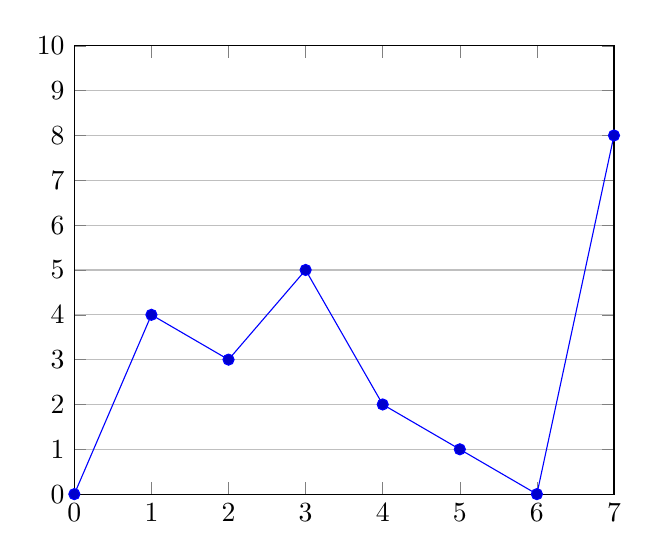
\begin{tikzpicture}
\begin{axis}[
xmin=0, xmax=7,
ymin=0, ymax=10,
xtick={0,1,2,3,4,5,6,7},
ytick={0,1,2,3,4,5,6,7,8,9,10},
ymajorgrids=true,
]
\addplot coordinates{(0,0)(1,4)(2,3)(3,5)(4,2)(5,1)(6,0)(7,8)};
\end{axis}
\end{tikzpicture}
```

* xmin, ymin, xmax, ymax 這些是指定 x 軸與 y 軸的最大、最小值
* xtick, ytick 是指定 x 軸與 y 軸上的標記的位置
* ymajorgrids 是繪製出與 y 軸相交的格線,可以用 xmajorgrids 來繪製出與 x 軸相交的格線,或用 grids=major 同時繪製兩者。

###長條圖

長條圖與折線圖有者異曲同工之妙

```latex
\begin{tikzpicture}
\begin{axis}[ybar, ybar interval=0.75, enlargelimits=0.1]
\addplot coordinates{(2040,9.50)(2030,10.60) (2020,12.58)};
\addplot coordinates{(2020,17.50) (2030,24.10) (2040,30.60)};
\legend{0~14歲人口所占比率(\%),65歲以上人口所占比率(\%)}
\end{axis}
\end{tikzpicture}
```

* ybar 指的是長條與 y 軸平行,另外還有 xbar 這個選項可以用。
* ybar interval 是指定長條之間的空隙,1 代表沒有空隙。
* enlarge limits 是調整整個座標軸與圖表的元素間的距離,另外也可以用enlarge x limits, enlarge y limits 等等來單獨調整特定的座標軸。

###散佈圖

散佈圖也很簡單。

```latex
\begin{tikzpicture}
\begin{axis}
\addplot[scatter, mark=*, only marks]
coordinates{(143,62) (50,594) (165,53) (139,348) (145,194) (75,533) (51,258) (154,492)};
\end{axis}
\end{tikzpicture}
```

* scatter 是讓顏色依據 y 軸的數值而變化
* only marks 是不讓點之間用線連起來
* mark 是指定點的標記的樣式

###從其他檔案輸入數據

上面的方法這只適用於數據只有寥寥幾筆時,不然如果有一千多筆,一個一個 key 未免太過勞神費力,不過 pgfplots 都幫你想好了,他可以讓你從 .dat 或 .csv 檔中輸入數據。

```latex
\begin{tikzpicture}
\begin{axis}[x tick label style={/pgf/number format/1000 sep=},width=10cm, grid=major]
\addplot table [x=year, y=youth, col sep=comma, mark=none] {data.csv};
\addlegendentry{0~14歲人口所占比率(\%)}
\addplot table [x=year, y=old, col sep=comma, mark=none] {data.csv};
\addlegendentry{65歲以上人口所占比率(\%)}
%\addplot table[meta=mid]{output.dat};
\end{axis}
\end{tikzpicture}
```

* x tick label style 是調整 x 軸上標示的樣式。
* table 是表示資料來源是類似表格的形式。
* x=, y= 是指定 x, y 的數據要從哪一欄輸入。
* col sep 是告訴 pgfplots 欄與欄的分界是用什麼符號。

##三維圖形

終於進入三維圖形了,

\end{markdown}\newpage
\input{24}\newpage
\begin{markdown}
#30天 LaTeX 挑戰 Day 25 biblatex

------

biblatex 是一個管理參考文獻的 package,他可以幫助我們方便快速的管理參考文獻。

##前置作業

首先我們需要準備 .bib 檔, .bib 檔的基礎形式如下

```latex
@Article{key,
author = {作者},
title = {標題},
journal = {期刊},
year = {年份},
}
```


`@Article` 是宣告參考文獻是期刊中的文章,key 是在文章中引用連結使用的,但通常我們不用親自撰寫 .bib 檔,因為像 Google Scholar 之類的文獻資料庫都會提供 bibtex 的格式。

圖片

上圖是如何在 Google Scholar 取得 .bib 檔的方式。

##基礎使用

在準備好 .bib 檔後就可以開始使用 biblatex 了,首先我們需要告訴 biblatex 我們的 .bib 檔叫什麼名字。

```latex
%\usepackage{biblatex}
\addbibresource{name.bib}
```

利用 `\addbibresource{•}` 告訴 biblatex .bib 檔的名稱後,我們就可以利用 `\cite{key}` 在文章中引用參考文獻了。

```latex
Free software 跟價錢並沒有關係,這裡的 Free 指的是自由。\cite{stallman2002free}
```

如果不是使用 overleaf 的人需要注意,我們需要額外跑一次 bibber 和兩次 LaTeX,順序如下:

1. LaTeX
2. biber
3. LaTeX 
4. LaTeX

這樣就可以引用參考文獻了,但我們還需要用 `\printbibliography` 將有用到的參考資料都列出來。

```latex
\printbibliography
```

這樣所有被引用過的資料就都被列出來了,如果有參考文獻沒有被直接引用,又想要讓他出現在此,需要用 `\nocite{key}` 將他列出來。

```latex
Free software 跟價錢並沒有關係,這裡的 Free 指的是自由。\cite{stallman2002free}
\nocite{key}
\printbibliography
```

如果想將檔案中所有的參考文獻都列出,只需將 key 換成 * 就好了,如果引用了許多文章,但最後在列出時想要分類這一大群的參考文獻時,有兩種方法,第一種是利用 `type=` 來依照參考文獻的類型分類。

```latex
\printbibliography[type=article, title=article]
\printbibliography[type=book, title=book]
```

第二個方法是在撰寫 bib 檔時加入 `keywords` ,以便分類。

```latex
\printbibliography[keyword=LaTeX, title=article]
\printbibliography[keyword=Overleaf, title=book]
```

```latex
@book{stallman2002free,
  title={Free software, free society: Selected essays of Richard M. Stallman},
  author={Stallman, Richard},
  year={2002},
  publisher={Lulu. com},
  keywords={}
}
```

如果想要更進一步的了解 biblatex 到底可以做什麼,可以參考以下幾篇文章。

\end{markdown}\newpage
\input{26}\newpage
\begin{markdown}
#30天 LaTeX 挑戰 Day 27 lualatex

------

Lualatex 是將 Lua 與 TeX 結合在一起,讓改動 TeX 的排版規則時可以不用 TeXing,更詳細的使用需要對 LuaTeX 與 LaTeX 有深刻的認識,目前我的能力還不到這麼深厚,所以我只介紹一些基礎的用法。

## 基礎用法

想要在 LuaLaTeX 裡使用 Lua 需要透過 `\directlua{}` 的協助,這個命令會將花括號中命令轉給 Lua 解釋器,要想讓 Lua 產出的結果可以轉回給 LaTeX 需要用 `tex.sprint`。

```lua
tex.sprint("$\cos(0)$等於".. math.cos(math.rad(0)))
```

執行之後可以看到 $\cos$ 被輸出出來了,這就是基礎的 LuaLaTeX 的用法更進階的也可以將 for 迴圈帶入使用

```lua
\directlua{
tex.sprint("\\begin{tabular}{|c|c|c|}")
tex.sprint("\\hline")
tex.sprint("x & sin(x) & cos(x) \\\\ ")
tex.sprint("\\hline")
for x = 0,180,10 do
	tex.sprint(x .." & ".. math.sin(math.rad(x)) .." & ".. math.cos(math.rad(x)) .." \\\\ ")
	tex.sprint("\\hline")
end
tex.sprint("\\end{tabular}")
}
```

執行後可以看到有表格被產出了,如果有什麼重複性高的指令,也可以用這種方式來節省時間,這是基礎的 LuaLaTeX 的使用方法。

## 進階使用

進階使用我也不會所以在這裡放一個我看到的例子:

```lua
function fadelines(head)
        GLYPH = node.id("glyph")
        WHAT = node.id("whatsit")
        COL = node.subtype("pdf_colorstack")
        colorize = node.new(WHAT,COL)
        cvalue = 0
        for line in node.traverse_id(GLYPH,head) do
            colorize.data = cvalue.." "..1 - cvalue.." .5".." rg"
            node.insert_before(head, line, node.copy(colorize))
            cvalue = math.min(cvalue + .0008, 1)
        end
        return head
    end

    luatexbase.add_to_callback("pre_linebreak_filter", fadelines, "fadelines")
```

這樣產生的結果如下圖:

要達成這種效果,需要對 LuaLaTeX 以及 LaTeX 有著即為深厚的認識。

\end{markdown}\newpage
\begin{markdown}
#30天 LaTeX 挑戰 Day 28 用 LuaLaTeX 做動畫
\end{markdown}\newpage
\input{29}\newpage
\input{30}\newpage
\setlength{\parindent}{20pt}
\begin{markdown}
#30天 LaTeX 挑戰 Day 31 Beyond LaTeX

-------

30 天的挑戰終於過去了,我也算是用另一種方式成為了勇者,當初會想寫下這系列的文章可說全部都是意外,事情得要從一個地科作業開始說起,當時在寫地科作業的我正被「如何在 page 內加入數學方程式」而困擾著,於是我打開了 page 內建的插入方程式功能,只見一行大字出現在視窗內「請使用 mathml 或 LaTeX 來插入數學方程式」,這就是我遇見 LaTeX 的過程。

後來我就開始學習 LaTeX ,在學習的過程中我發現跟 LaTeX 有關的中文資料只有兩種,不是簡體字就是有一定年份的資料,除了這之外就全部都是英文資料了,雖然雙語能力固然重要,但沒有中文資料真的太慘了,所以我就下定決心要留點資料,那時剛好看到了鐵人賽,於是便下定決心要做這件事情。

\end{markdown}

\end{document}